\documentclass{beamer}

\usepackage[utf8]{inputenc}
\usepackage{float}
\usepackage{graphicx}
\graphicspath{{./pics}}
\usepackage{comment}
\usepackage{blindtext}
\usepackage{tabularx}
\usepackage{amsmath}
\usepackage{dsfont}
\usepackage{amssymb}
\usepackage{mathtools}
\usepackage{bm}
\usepackage{textcomp}
\usepackage{anysize}
\usepackage{listings}
\usepackage{color}
\usepackage{colortbl}
\usepackage{xcolor}
\usepackage{booktabs}
\usepackage{array}
\usepackage{dcolumn}
\usepackage{longtable}
\usepackage{multirow}
\usepackage{setspace}
\usepackage{caption}
\usepackage{subcaption}
\usepackage[hidelinks]{hyperref}
\usepackage{csquotes}
\usepackage{siunitx}
\usepackage{mathabx}
\usepackage{titlesec}
\usepackage[11pt]{moresize}
\usepackage{tocloft}
\usepackage{physics}
\usepackage{enumitem}
\usepackage{slashed}
\usepackage{cancel}
\usepackage{fancyhdr}
\usepackage[backend=biber]{biblatex}
\usepackage{lmodern}
\usepackage{lipsum}
\usepackage[T1]{fontenc}

\usetheme{Madrid}
\title[QFT on a Highly Symmetric Lattice]{Quantum Field Theory on a Highly Symmetric Lattice}
%\subtitle{}
\author{Marco Aliberti}
\institute[]{Università degli Studi di Torino}
%\date{\today}
\date{\formatdate{23}{10}{2023}}

\setbeamertemplate{navigation symbols}{} % Uncomment to remove navigation buttons

\addbibresource{Bibliography.bib}

\graphicspath{{./pics}}

\newcommand{\pr}[1]{\left(#1\right)}
\newcommand{\prs}[1]{\left[#1\right]}
\newcommand{\prc}[1]{\left\{#1\right\}}
\newcommand{\C}{\mathbb{C}}
\newcommand{\R}{\mathbb{R}}
\newcommand{\Z}{\mathbb{Z}}
\newcommand{\dV}{\int\dd^4x}
\newcommand{\id}{\mathds{1}}
\newcommand{\degree}{^\circ}

\let\oldCite\cite
\renewcommand{\cite}[1]{\textsuperscript{[\oldCite{#1}]}}
\renewcommand*{\nameyeardelim}{\addcomma\space}


\begin{document}

\begin{frame}
  \titlepage
\end{frame}

\begin{frame}
  \frametitle{Why Lattice Quantum Chromodynamics?}
  \centering
  In quantum field theory scattering amplitudes in the form
  \begin{equation*}
    \bra{f}\ket{i} = \int_{\phi_i}^{\phi_f}\mathcal{D}\prs{\phi} e^{-S[\phi]}
  \end{equation*}
  need to be evaluated.
\onslide<2->
  There are two possible approaches:
  \vspace{\baselineskip}
  \begin{columns}[t]
    \column{0.5\textwidth}
    \centering
    Perturbative\\
    \vspace{\baselineskip}
    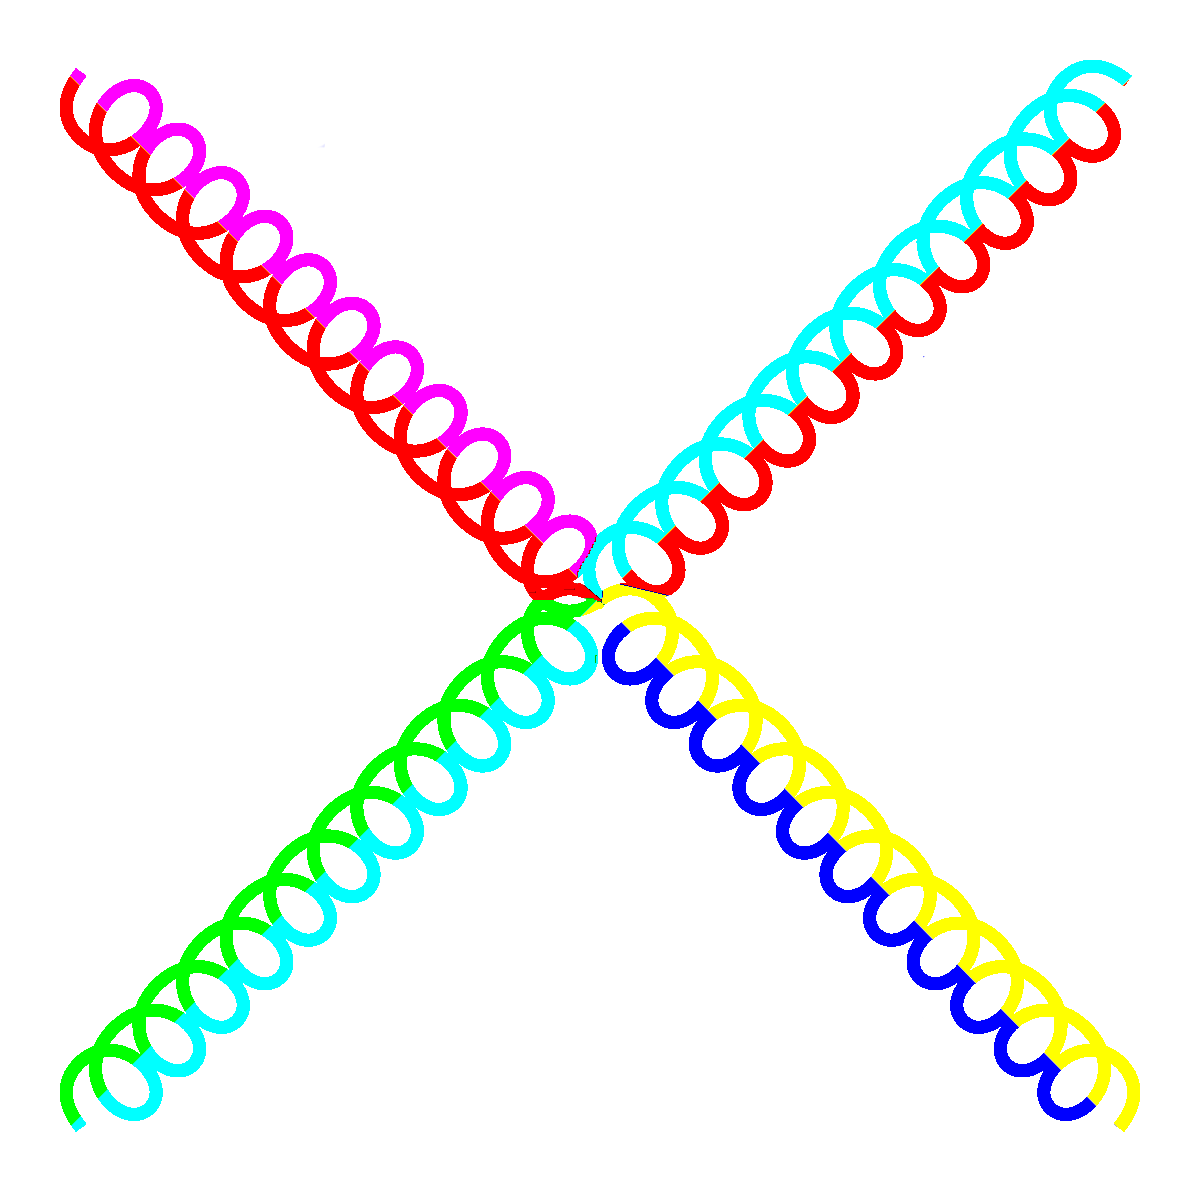
\includegraphics[width=0.4\textwidth]{gluonfd.png}
    \column{0.5\textwidth}
\onslide<3->
    \centering
    Non-Perturbative\\
    \vspace{\baselineskip}
    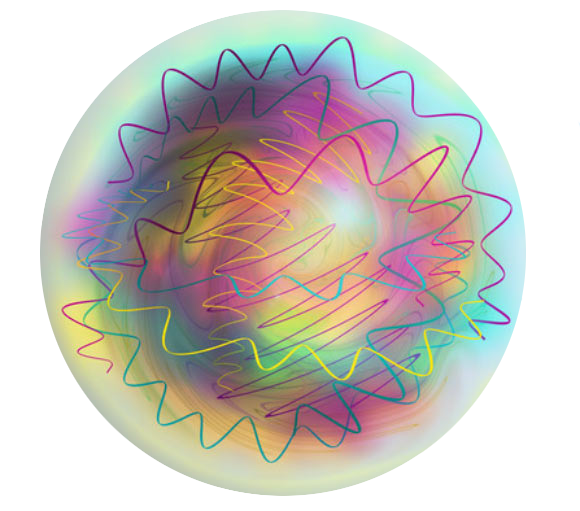
\includegraphics[width=0.45\textwidth]{Glueball.png}
  \end{columns}
\end{frame}

\begin{frame}
  \frametitle{Perturbative vs Non-Perturbative}
  \centering
  \begin{columns}[t]
    \column{0.5\textwidth}
    \centering
\onslide<1->
    Perturbative\\
    \vspace{0.5\baselineskip}
    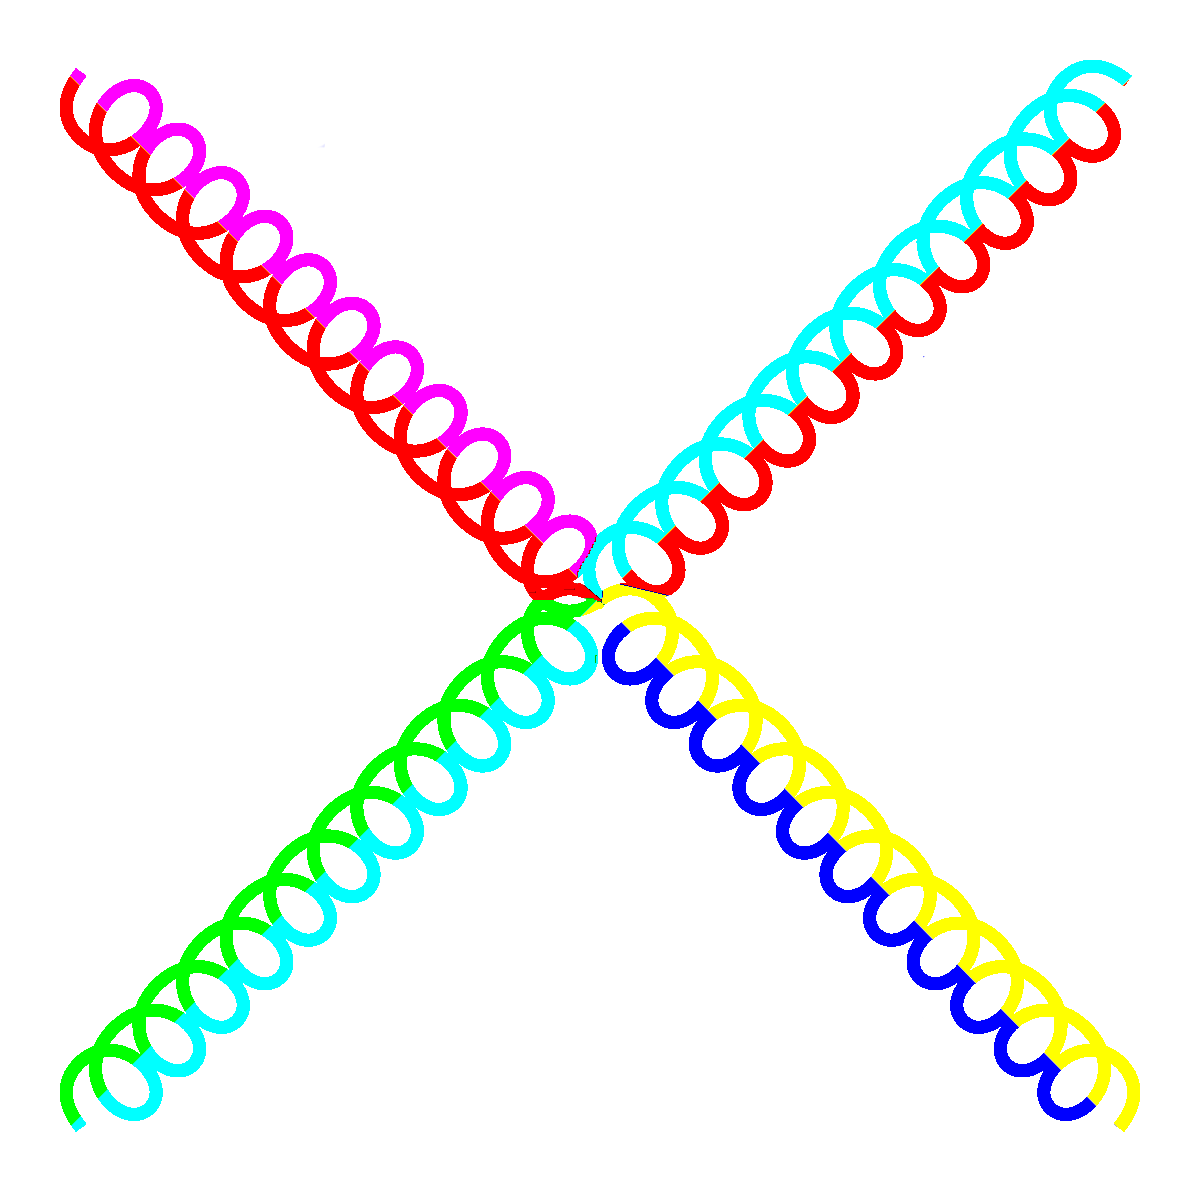
\includegraphics[height=0.4\textwidth]{gluonfd.png}\\
    \vspace{0.5\baselineskip}
    \begin{itemize}
     \item Straightforward series expansion in powers of small $g$ $\Leftrightarrow$ Feynman diagrams with $n$ loops
\onslide<2->
     \item UV divergencies need to be eliminated
\onslide<3->
     \item Fails predicting quantities with essential singularities as $g\rightarrow0$
    \end{itemize}
    \column{0.5\textwidth}
    \centering
\onslide<1->
    Non-Perturbative\\
    \vspace{0.5\baselineskip}
    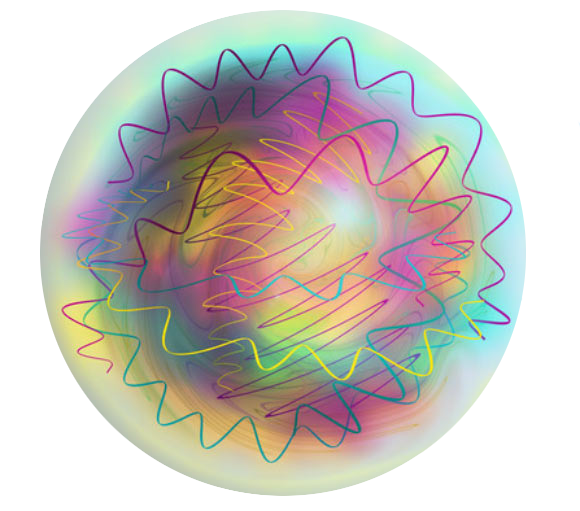
\includegraphics[height=0.4\textwidth]{Glueball.png}\\
    \vspace{0.5\baselineskip}
    \begin{itemize}
\onslide<4->
     \item No straightforward approach
\onslide<5->
     \item Can have a natural cut-off for high momenta $\Rightarrow$ No UV divergencies
\onslide<6->
     \item Can predict quantities with essential singularities as $g\rightarrow0$
    \end{itemize}
  \end{columns}
\end{frame}

\begin{frame}
  \frametitle{Lattice Field Theory}
\end{frame}


\end{document}
